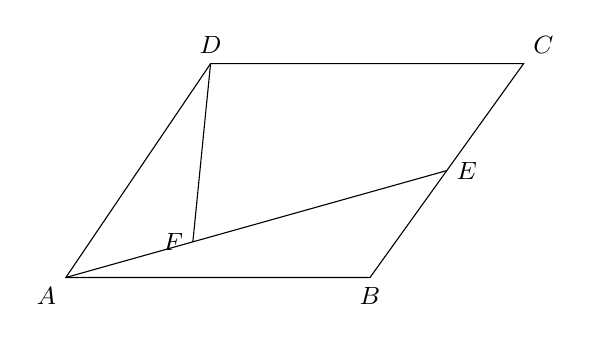
\begin{tikzpicture}[scale=.75, every node/.style={font=\small}]
  \coordinate (A) at (0,0); \coordinate (B) at (5.15,0);
  \coordinate (C) at (7.75,3.62); \coordinate (D) at (2.45,3.62);
  \coordinate (E) at (6.45,1.81); \coordinate (F) at (2.15,.60);
  \draw (A)--(B)--(C)--(D)--cycle;
  \draw (A)--(E); \draw (D)--(F);
  \node[below left] at (A) {$A$};
  \node[below] at (B) {$B$};
  \node[above right] at (C) {$C$};
  \node[above] at (D) {$D$};
  \node[right] at (E) {$E$};
  \node[left] at (F) {$F$};
\end{tikzpicture}
